\begin{figure}[htbp]

\begin{center}
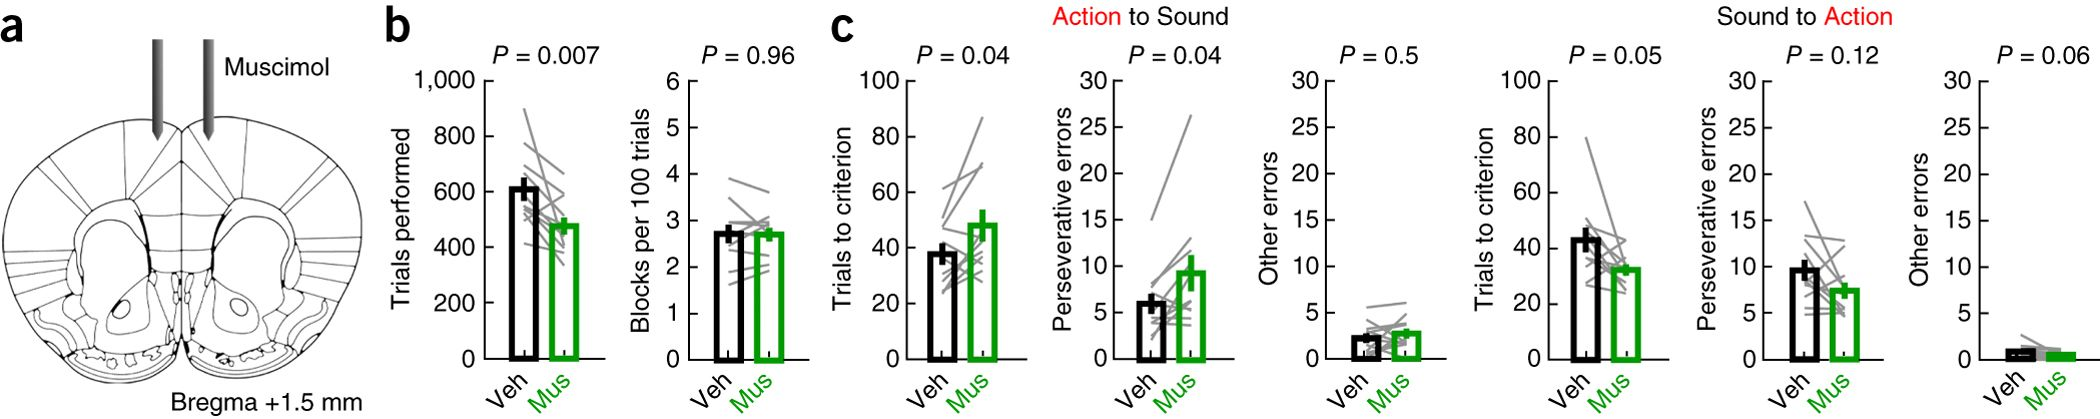
\includegraphics[width=\textwidth]{Figures/Chapter3/NN_fig2} 
\end{center}

\caption[Bilateral inactivation of M2 impaired adjustment to sound rule]
{Bilateral inactivation of secondary motor cortex (M2) impaired adjustment to sound-guided trials. (a) Schematic of experiment. (b) Task performance after bilateral infusion of saline vehicle (Veh) or muscimol (Mus) into M2. (c) Effects of muscimol infusion on action-to-sound and sound-to-action rule shifts. Gray lines, individual paired experiments. Bars, $\mathit{mean}\pm\mathit{SEM}$. Wilcoxon signed-rank test, action-to-sound: trials to criterion, $p = 0.042$, $W = 10$; perseverative errors, $p = 0.042$, $W = 10$; other errors, $p = 0.5$, $W = 24$. Sound-to-action: trials to criterion, $p = 0.054$, $W = 55$; perseverative errors, $p = 0.12$, $W = 51$; other errors, $p = 0.06$, $W = 46$. $N = 11$ mice.}

\label{fig:NN_fig2}
\end{figure}